\chapter{On Mobile Analytics}~\label{chapter-on-mobile-analytics}
Mobile Analytics is a specialisation of a general category of software usage analytics and some aspects are in-common. Nonetheless it is distinct and has unique characteristics based on the operating system, the ways libraries are bundled with apps, etc. TBC.

Mobile Analytics, an umbrella term that encompasses various aspects of:
\begin{itemize}
    \item Products and/or Services:
    \item Software libraries:
    \item Data reporting, filtering, collection, propagation, import, storage, analysis, reporting, export
    \item Data use and ownership, data 'protection', privacy, sensitive data, permissions, etc.
    \item Types and extent of data collected, and not collected (which affects the ability to analyse, fault-find, etc.)
    \item The history and movements in the industry might also be relevant and of interest.
\end{itemize}

Include my 3 layers figure. Perhaps the 3 views of quality figure. My data sources figure. 

\section{Layers of an app}
\begin{enumerate}
    \item User Interface:
    \item The rest of the app:
    \item The platform's perspective of an app:
\end{enumerate}


\section{Designing the content/messages} 
% I'm not sure whether content or messages, or a mix of both words, best encompasses the topic I wish to discuss here. Messages can have content, however sometimes a message is a message by its existence, even with no payload. (2 rings on the home phone when you arrive, told the family you'd arrived without needing to pay for the telephone call. Heartbeat messages in systems, etc.). Also the design may include non-content aspects, content transformations, etc. Anyway, let's get writing. 
This section applies to messages that an app could emit regardless of the conduit (\emph{i.e.} it applies to logging and using mobile analytics). At the risk of some ambiguity, the term log will be used to reflect both logging and mobile analytics in this section to improve overall readability.

\emph{Related concepts}: The uneven U, computer protocols (layers, formatting, and contents), structured messages, what to log. %MUST-DO expand this section.

There are many choices that can be considered in terms of designing the content/messages. For various reasons developers may pay little strategic attention to logging in their daily work. For those who do choose to consider logging strategically there are various considerations, including:
What to log, how to log, where to log, data transformations, delivery mechanisms and characteristics.

Developers have control over what to log, how, and when to generate the log messages. They may be constrained in various ways by APIs, message lengths, encoding, and formats, access to messages, and when messages will be transmitted, \emph{etc.} 

It is possible to test the constraints, for instance by writing custom automated tests and/or apps that generate a variety of messages where the outputs are checked somehow. The checking may be partly or completely performed programmatically (we did some unpublished research in this area in 2018).

The purpose of the message may differ in the type and level of information it is intended to convey. Some messages may contain low-level, or detailed, error messages intended to help improve the technical aspects of the software to make the software more robust. Other messages may aim to communicate intent, completion of a task, activity or user-journey in the software. For example, IBM published a paper about software called CX Mobile that aims to record and visualise user journeys for iOS and Android apps~\cite{hu_tealeaf_cxmobile}.


The distinction between analytics and logging may be murky. A pragmatic heuristic is to use the declared category of the library, tool or service, for instance Firebase analytics would be considered as analytics whereas Timber.io would be considered as logging even though both contain aspects of the other category.

Similar to the concept of black box testing (where software's behaviour is observed and assessed without knowing the internals), external software can observe the behaviours of apps. Google have developed and integrated software that monitors apps running in Google approved versions of Android. The data is collected per device and provided automatically to Google servers if the device has the relevant settings enabled~\cite{google_play_share_usage_and_diagnostics_info_with_google}. This data is processed by Google who provide some portions of the data to the registered developers of that app in the Google Play Store.

\emph{Idea for expansion:} Drop-off in data for a population  c.f. marketing funnels, funnels for shopping carts, etc.

% Mobile Developer's Guide to the fifth dimension
% available from https://www.dropbox.com/s/no70z2hiod6z7o8/Fifth_Dimension_v1.pdf?dl=0 (took 20 - 30 mins to track down)

\section{The mechanics of sending data}
To be useful the analytics data needs to reach the system that processes, analyses and reports on it. There are various mechanisms that can be used to send data ranging from unlikely (at least for the app store ecosystems and their apps), retyping, transferring using USB devices, etc. to the most likely which uses a valid internet connection over WiFi or a mobile network. 

MUST-DO expand the following lists.
\begin{itemize}
    \item Triggers, batching, caps/buffers/limits, availability of any connection, or only approved connection, priorities, latency, delays,
    \item Permissions (including permissions to access the source data on the device and permission to share it (and permission to use certain connections/times/etc.)
    \item authorisation and authentication, spoofing and poisoning,
    \item freshness|staleness of the data, encoding, ...
    \item Lean data, privacy and sensitivity of the contents, data quality, encoding, ...
    \item Screening and filtering: who, when, how, why.
\end{itemize}

Examples:
\begin{itemize}
    \item Fabric Crashlytics, batching and caps/limits.
    \item Mozilla Glean telemetry.
    \item MQTT~\citep{adil2020_sending_logs_from_flutter_apps}

    
\end{itemize}

Wayne Chang, one of the co-founders of Crashlytics, wrote about the genesis of Crashlytics from 2011 to 2013~\citep{chang2015_how_six_people_built_crashlytics}. The started was created to develop ``an SDK that would make it easier for app developers to uncover why their apps were crashing." %They realised their SDK also collected normal analytics data.
Twitter acquired the startup, their first of the acquisitions of Crashlytics. Once they knew their crash reporting library met the needs of developers they devised a mobile analytics that would provide answers to developers of mobile apps. They called the mobile analytics product: ~\emph{Answers}. Their product became a tremendous success with developers, and `Answers' grew to handling 5 billion events every day, in real-time, within 7 months of the launch of the service~\citep{chang2015_how_six_people_built_crashlytics, twitter2015_edsolovey_handling_5B_sessions_a_day_in_real_time}. These became integrated in a service called \href{https://fabric.io}{fabric.io}~\footnote{Now owned and operated by Google~\url{https://firebase.google.com/}.} One of the goals of Fabric was to use \emph{``Crashlytics data in a way that saves developers from information overload or “analysis paralysis”."}~\citep{burke2014_wayne_chang_interview}. 
% https://www.siliconrepublic.com/play/the-interview-wayne-chang-crashlytics-co-founder-and-now-twitter-developer-lead

%%% More material available at the following if it's worth expanding this topic.
% https://twitter.com/answersio "Answers is the analytics engine that powers the Fabric platform."
% https://thenextweb.com/twitter/2014/07/15/crashlytics-answers/
% https://youtu.be/G1LrMXR3Zko Twitter Flight 2015 - A Deep Dive into the Answers Backend by Ed Solovey
% Part of Twitter Flight 2015 - Mobile Track https://www.youtube.com/playlist?list=PLFKjcMIU2WsjRto4UpcU_k3ESIY-XOSi6


\section{Designing the analytics platform}
When Twitter owned and operated Crashlytics their service handled five billion sessions per day in 2015. They designed designed the device to server communication to reduce the bandwidth and network usage and batched the data. They stored the events of the device until it was safely transmitted. And to minimise latency of the data arriving various client-side triggers attempted to send data quickly yet without adversely affecting the user-experience~\citep{twitter2015_edsolovey_handling_5B_sessions_a_day_in_real_time}.

In a video recording on YouTube~\citep{twitterdev2015_a_deep_dive_into_the_answers_backend}, the same employee Ed Solovey, describes how they designed the backend architecture of their online analytics service, Answers, at Twitter's conference `Twitter Flight 2015'. This conference was aimed at developers, and this talk one of six they provided in the Mobile Track.

\begin{itemize}
    \item Lambda Architecture included parallel batch and realtime layers. The realtime layer was covered in this YouTube talk.
    \item Ideal: linear scaling in \# of events, together with key challenges: 
    \begin{itemize}
        \item Daily Active Users - Cardinality: They needed a set that holds millions of members,
        \item Retention - Set membership: They needed multiple sets that hold thousands of members each: these were calculated for D30, D7, and D1 (30, 7 and 1 day) daily active usage,
        \item Session Duration - Median of millions of data points. They needed a sorted list of millions of data points.
    \end{itemize}
    \item Probabilistic Data Structures: a very small tradeoff in accuracy loss to provide a huge gain in space or time complexity. They wanted space savings:
    \begin{itemize}
        \item \emph{Hyper Log Log}~\citep{flajolet2007_hyper_log_log, heule2013_hyper_log_log_in_practice} which they used to track daily active users. It uses \nth{1000} of the space of a brute force approach. The loss in accuracy is less than 1\%.
        \item \emph{Bloom Filter} is used to track retention and set membership. It uses \nth{100} of the memory with less than 1\% error rate. The calculation is much more granular than tracking daily active users and therefore the reduction in memory use is smaller,
        \item \emph{Session Duration} - they created their own algorithm which reduced memory use to \nth{500} of the brute force approach, with less than 1\% error rate.
    \end{itemize}
    
\end{itemize}



\subsection{Visual (GUI-level) analytics}

\subsubsection{A potted-history of related work}
When Android was publicly launched in 2008, a team of Google engineers, including myself, developed various utilities and applications to help make Android more useful and usable for people with visual impairments. The project became known as the \emph{eyes-free} project and the source code was released as the, now archived, \href{https://code.google.com/archive/p/eyes-free/}{\texttt{eyes-free}} opensource project. 

A key aspect of that work was the implementation of code that 'overlaid' the user interface within an app and intercepted touch events Android sent to the app in response to user interactions with the touch screen. The library and apps were presented by various Google engineers at the time, for instance by T.V. Raman and Charles Chen at Google I/O 2009~\footnote{ \href{http://transcriptvids.com/v/xS-ju61vOQw.html}{link to the video with transcription} for ease of searching for the overlay~\texttt{TouchGestureControlOverlay}. The slides are available at~\url{https://docs.huihoo.com/google/io/2009/Th_0115_EyesFreeUserInteraction.pdf} and a version of the library in one of my also archived projects~\href{https://github.com/julianharty/android-daisy-epub-reader/blob/master/src/com/google/marvin/widget/GestureOverlay.java}{\texttt{GestureOverlay} in Android DAISY ePub Reader}.} 

I am not aware of any work that extended our work at the time, however I believe it would be practical to extend that code to include GUI-level analytics by reporting the touch events, together with some basic information about the app version, device model, settings, and screen orientation to be able to use the event data.

Eventually the Android operating system included Accessibility APIs and incorporated Text-To-Speech (TTS) support directly, for instance the popular~\href{https://support.google.com/accessibility/android/answer/6283677?hl=en}{TalkBack Screen Reader}. In tandem several commercial companies released TTS 'engines', which meant the apps and utilities the team had developed became less necessary. In summary our work started with providing a custom overlay that developers incorporated into their app, and became less relevant once the platform had sufficient support for Accessibility.

%SHOULD_DO discuss heatmapping tools for non-mobile platforms e.g. web, and perhaps even desktop. Also cite relevant research. 

\subsubsection{Heatmapping for mobile apps}
%MUST_DO Include examples from AppSee that were in the mobile analytics playbook.

% SHOULD_DO combine these figures as sub-figures. Trim whitespace on Azetone image.
\begin{figure}[htbp!]
    \begin{minipage}{\textwidth}
    \centering
    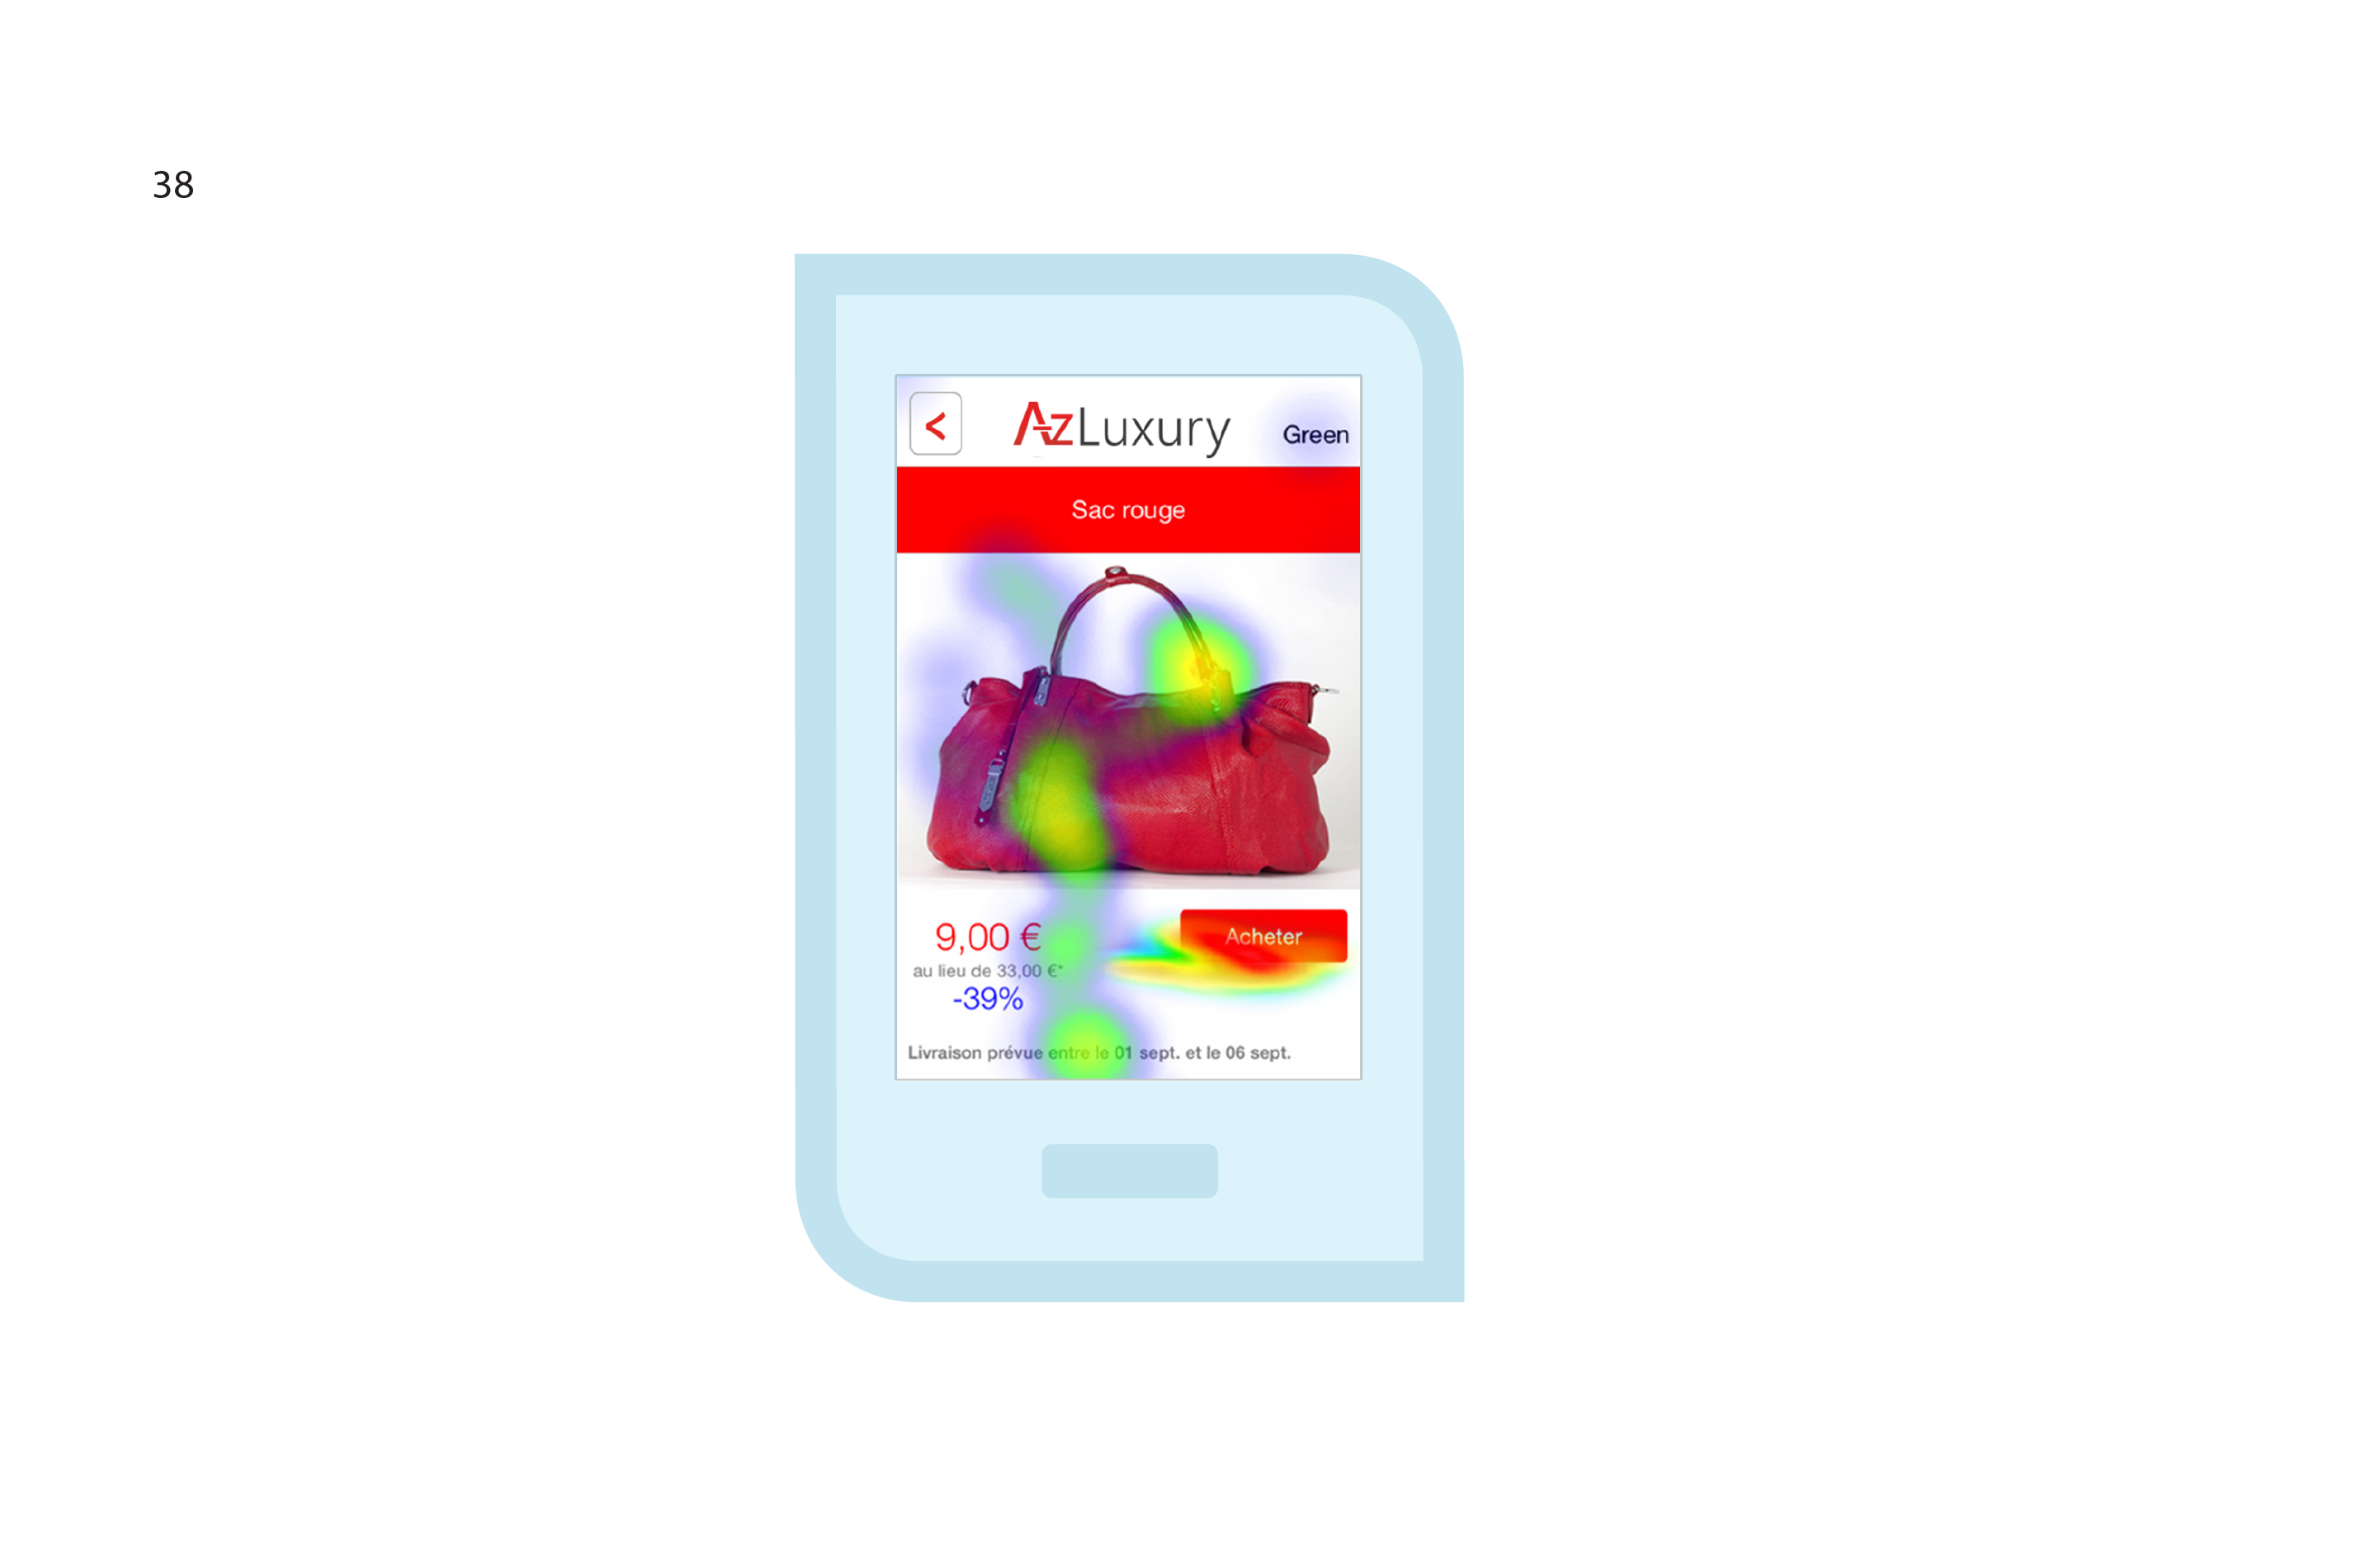
\includegraphics[width=10cm]{images/mobile-analytics-playbook/Chart-10-azetone.png}
    \caption[Example of Azetone heatmap overlaid on shopping app]{Example of Azetone heatmap overlaid on shopping app~\footnote{Image credit: First published in the Mobile Analytics Playbook~\cite{harty_aymer_playbook_2016}}.}
    \label{fig:azetone-heatmap-example}
    \end{minipage}
\end{figure}

\begin{figure}[htbp!]
    \begin{minipage}{\textwidth}
    \centering
    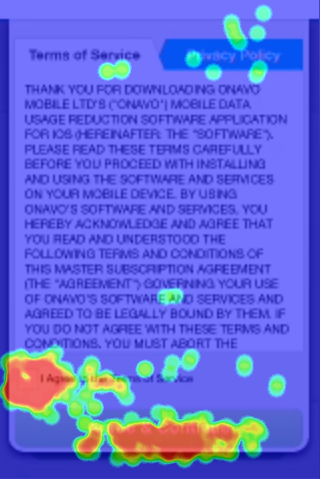
\includegraphics[width=8cm]{images/mobile-analytics-playbook/Appsee-Screen-Heatmap.png}
    \caption[Appsee example of usability flaw found using visual analytics]{Appsee example of usability flaw found using visual analytics~\footnote{Image credit: First published in the Mobile Analytics Playbook~\cite{harty_aymer_playbook_2016}}.}
    \label{fig:appsee-example-t-and-c-screen}
    \end{minipage}
\end{figure}

Learn more about Appsee's work: ~\url{https://www.youtube.com/watch?v=aRN_XrxNCNE}

~\url{https://www.youtube.com/watch?v=GQ2DoINkba4}

~\subsubsection{Extending GUI to Multimodal UI analytics}

\begin{figure}[htbp!]
    \begin{minipage}{\textwidth}
    \centering
    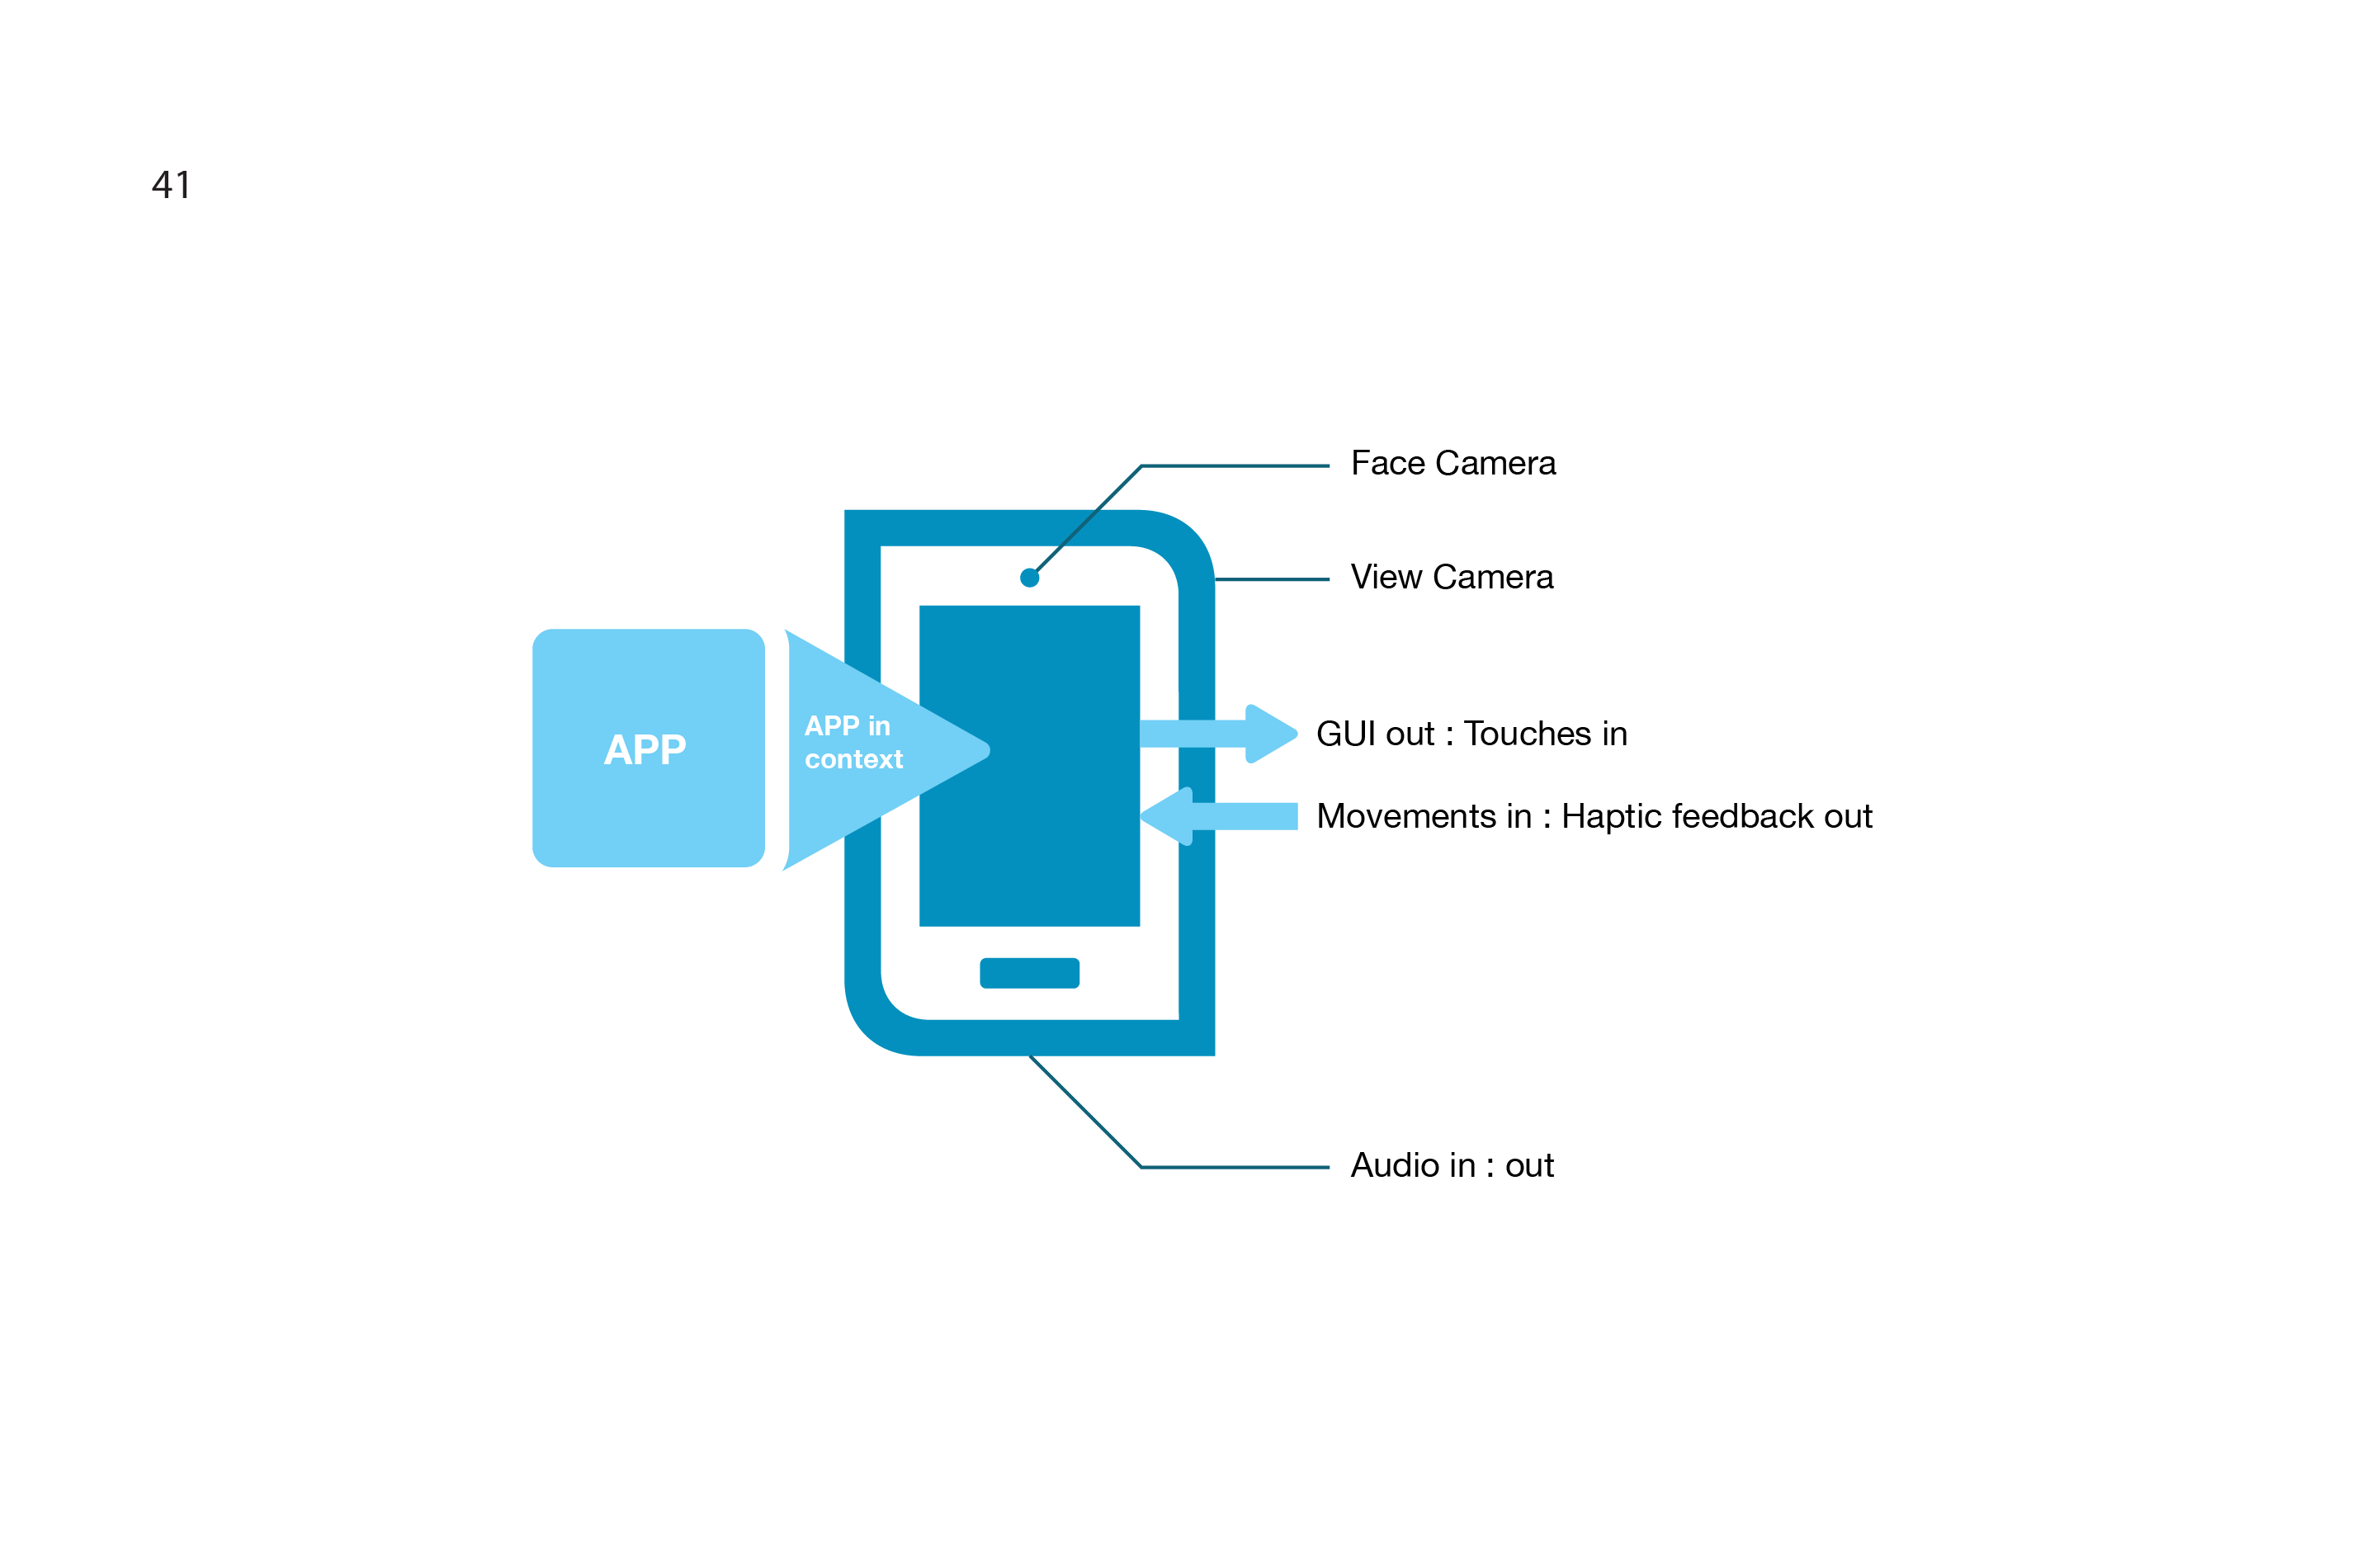
\includegraphics[width=15cm]{images/mobile-analytics-playbook/Chart-11-extending-gui-analytics.png}
    \caption[Extending GUI Analytics]{Extending GUI Analytics~\footnote{Image credit: First published in the Mobile Analytics Playbook~\cite{harty_aymer_playbook_2016}}.}
    \label{fig:extending-gui-analytics}
    \end{minipage}
\end{figure}
% https://texfaq.org/FAQ-ftncapt

\subsection{Platform-level analytics}~\label{platform-level-analytics}
Mobile software platforms include an operating system that runs on end-user devices such as smartphones and tablet devices. Operating systems are responsible for running software, including apps. They may also be responsible for stopping apps, for instance to recover from adverse conditions such as frozen apps (that are no longer responsive for the user), crashes (where the app does not handle the crash adequately), or to free up resources for other purposes. Mobile operating systems often incorporate one or more centralised log buffers~\footnote{Buffers are also often called files in the context of logging, buffers have a finite storage and older events are eventually overwritten.}, when application software writes log messages % SHOULD-DO check the following: or to STDOUT (the standard output stream used by traditional programs and still available to apps)
using the platform logging APIs (\emph{e.g.}~\texttt{android.util.log}) and other logging APIs which use this indirectly these log messages are recorded in a centralised log. For Android there are currently five documented log buffers (radio, events, main, system, crash)~\footnote{~\url{https://developer.android.com/studio/command-line/logcat\#alternativeBuffers}}. Developers do not choose which buffer is used, the Android operating system determines which log to use, for instance the crash buffer, perhaps unsurprisingly is used to record crashes.

Trusted (privileged) software may be granted access to one of more of these device-wide logs (early releases of Android allowed any app to access them with permission~\footnote{Examples of apps that had access and details of Android logs in earlier versions are described in~\url{https://android.stackexchange.com/questions/14430/how-can-i-view-and-examine-the-android-log}.}). What most users perceive as 'Android' is actually a combination of an operating system, Android, together with various software called Google Mobile Services (GMS) Google provides to approved partners for certified devices~\footnote{\emph{``Google Mobile Services (GMS) is a collection of Google applications and APIs that help support functionality across devices. These apps work together seamlessly to ensure that your device provides a great user experience right out of the box."}~\url{https://www.android.com/gms/}}. GMS includes Google Play and various APIs including some related to Google Play~\footnote{~\url{https://developers.google.com/android/guides/overview} and~\url{https://developers.google.com/android/guides/setup}}.

A seemingly logical design for Google to collect device-level analytics is through a combination of some software packaged as part of GMS that has privileged access to read the relevant device logs. The logs include the data that is also reported in Google's Android Vitals service (part of Google Play Console). Developers can read these logs locally using a combination of the Android Debug Bridge (adb) software to access the logs on devices that have been enabled in development mode and which have debugging enabled and authorised for the developer's computer. Google provide an API \texttt{android.app.usage}~\footnote{\href{https://developer.android.com/reference/android/app/usage/package-summary.html}{Documentation available at~\texttt{android.app.usage}}.} that provides access to various configuration, event, and usage statistics, amongst others.
% https://stackoverflow.com/questions/9012361/how-to-track-app-usage-in-android-how-to-detect-when-an-activity-is-launched

\subsubsection{iOS device analytics}
Apple ask clear direct questions of users and provide clear explanations (at least for those who understand the concepts). Their mobile devices ask users two questions when they first sign into a new release of iOS (on both new and updated devices):
\begin{itemize}
    \item \textbf{iPhone Analytics}: \emph{``Help Apple improve its products and services by allowing analytics of usage data from your iPhone. You can change your decision later in Settings. All data is collected using prvacy preserving techniques such as differential privacy and is not associated with you or your account."} The setting can be controlled via \texttt{Settings > Privacy > Analytics \& Improvements} and looking under \texttt{Analytics Data}.
    \item \textbf{App Analytics}: \emph{``Help app developers improve their apps by choosing to share app activity and crash data with them through Apple. You can change your decision later in Settings."} The setting can be controlled via: \texttt{Settings > Privacy > Analytics \& Improvements Share With App Developers}.
\end{itemize}

OSX: Data \& Privacy

\subsection{Mapping Analytics tools to layers of an app}

\subsection{Key components of Mobile Analytics}
\begin{itemize}
    \item [Local] Logging component, on device:
    \item Software that records pertinent data locally:
    \item Local data collector:
    \item Data transmitter:
    \item A Conduit:
    \item Data receiver:
    \item Load, validate, transform:
    \item Data base:
    \item Data processing (e.g. filtering, grouping and aggregation, pattern recognition and matching, etc.)
    \item Report Generator:
    \item User Interfaces, including APIs:
\end{itemize}

\subsubsection{Four perspectives on apps in a platform ecosystem}
\large{\texttt{\emph{1} Public \textbf{(}\emph{2} User \textbf{(}\emph{3} Development team \textbf{(}\emph{4} App Store\textbf{)))}}}
% To tweak the text size, see https://texblog.org/2012/08/29/changing-the-font-size-in-latex/

App stores have established various groups of people, each has a distinct view of the mobile apps in the app store. Broadly, the public (group 1) knows the least, and the app store (group 4) knows the most.

Groups and their perspectives:
\begin{enumerate}
    \item \textbf{Public}: The public can see information that is publicly available in the app store pertaining to apps. This information includes screenshots, descriptions, popularity, and additional information about particular apps. They may also see rankings, promoted apps, etc.
    \item \textbf{User}: A user has installed an app, they can explore the app and use it. They may form opinions on the usefulness, value and quality of the app. They determine whether they use it, and when. They may stop using it for whatever reason, and may uninstall the app. QoE and UX both pertain to user's and their perspectives of an app.
    \item \textbf{Development team}: The development team own the creation and development of an app. They may also maintain and support it. They may obtain information from various sources pertaining to the use of their app from their app's user-base. They choose what an app reports and to whom in terms of logging recorded by, and analytics sent by, the app.
    \item \textbf{App Store}: The app store has an aggregate perspective of all the apps in their app store (and also apps they have suspended or rejected).
\end{enumerate}

There are many factors that influence why install mobile apps. These include perceived risk, trust, perceived benefit amongst other factors~\cite{harris2016identifying}. Trust, in turn, includes several considerations - whether an app is trustworthy and whether the \emph{`app market has high integrity'}~\cite{harris2016identifying}.

\begin{figure}[htbp!]
    \centering
    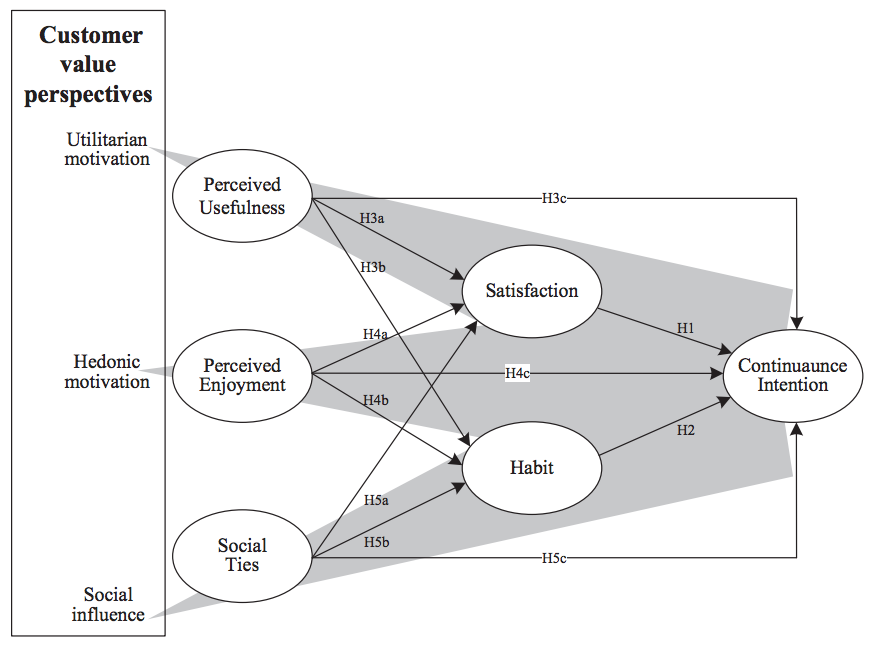
\includegraphics[width=13cm]{images/Consumer_Value_Perspectives_screenshot.png}
    \caption{Continuance Intention Research Framework (\textcopyright Elsevier Ltd 2015)}
    \label{fig:consumer_value_perspectives_elsevier}
\end{figure}
% Figure from: https://doi.org/10.1016/j.tele.2015.08.014
% RightsLink permission: 4836950640436 obtained 27 May 2020.

Users don't use all their apps, they use some because they're bored~\cite{pielot2015attention}, and others because they have to or want to. Uses and gratification of mobile apps by people in Jordan~\cite{ALNAWAS2016313}, and in the USA are assessed in detail in~\cite{gerlich2015app}. For apps that are used when people are bored they are easy to abandon, particularly if the quality of the app's performance is poor, for instance 35.18\% of users in~\cite{lim_investigating_country_differences} stated they abandoned apps because of crashes. 

Ongoing use may be longer for some categories of apps such as social apps~\cite{HSIAO2016342}, seasonal \emph{e.g.} Google's Santa Tracker app, periodic \emph{e.g.} a conference app for academic research conferences, and so on. Usage also varies by the type of app, for instance news apps may be used more in mornings, communications apps throughout the day, and games in the evenings~\cite{bohmer2011falling_asleep_with_angry_birds}. There are also differences in the behaviours of users from various countries~\cite{lim_investigating_country_differences}.  
\cite{HSIAO2016342} provides the research framework reproduced in Figure \ref{fig:consumer_value_perspectives_elsevier} ( used with permission)\footnote{RightsLink permission: 4836950640436 obtained 27 May 2020. DOI~\url{https://doi.org/10.1016/j.tele.2015.08.014}}) to help assess user's intentions to continue using an app.

Uninstalls: TBC see~\cite{bohmer2011falling_asleep_with_angry_birds} in turn cited in~\cite{lim_investigating_country_differences} on uninstalls. % MUST-DO complete this section 27-May-2020.

\begin{figure}[htbp!]
    \centering
    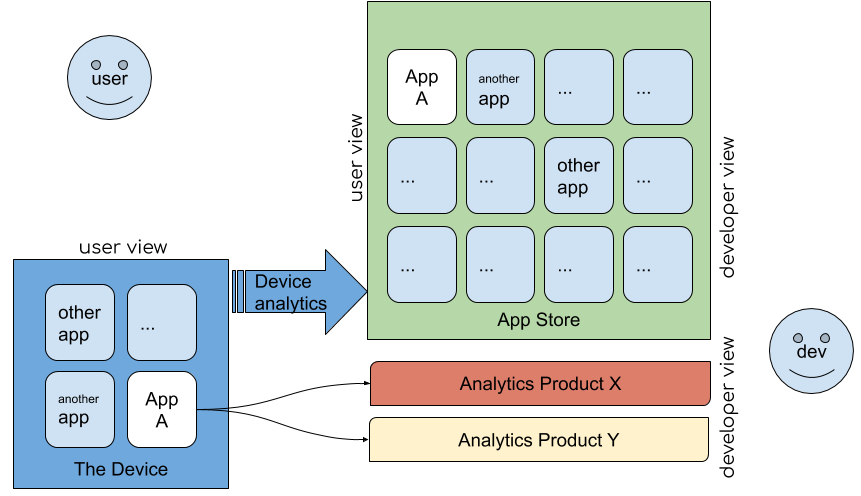
\includegraphics[width=\textwidth]{images/data_sources_and_views_25_jan_2020.jpg}
    \caption{Data sources and views}
    \label{fig:data_sources_and_views}
\end{figure}

Data can be collected by apps, devices, and the app store, as illustrated in Figure \ref{fig:data_sources_and_views}. Users can see which apps they have installed on their device and may be able to decide whether device analytics is collected. They can also see publicly available information about apps in the app store. Developers can see the same public data in the app store, they can also see additional data Google gathers and provides about \textit{their} apps together with whatever access they have to analytics tools incorporated into these apps.

Note: the third set of observers are the people and organisations who provide the app store and the various tools and products. They have a unique perspective across \textit{all the apps} that use their product. Google, for instance, calculates and publishes app-store wide "Bad behavior thresholds" for crash rates (1.09\%) and ANRs (0.47\%).

\section{Characteristics of Analytics Tools}


\begin{itemize}
    \item Status and Reporting of problems and outages
    \item Testability
    \item Performance Characteristics (Latency, Volumes,...)
    \item Time (Timezones, Daily Updates, Reporting periods, Data availability,...)
    \item Interoperability with external software e.g. for integration, analysis
    \item Vitality and Popularity: 
    \item Pricing:
    \item TBC
\end{itemize}

\section{Examples of flaws in mobile analytics offerings}
\subsection{Azetone [Heatmaps]}
Some quirks in the system at rest and never been used: as the following extract, in Figure \ref{fig:azetone_dashboard_flaws_for_kiwix_2015}, of a screenshot shows - a brand new account has some quirks that don’t seem correct:
\begin{itemize}
    \item The app structure at 0 is 33\% higher than last month
    \item For app structure and profiles set-up there is a bar, but not for the other indicators, which have none.
    \item Spurious percentages: 59\%, 29\% and 12\%
    \item 20 of 50,000 [users] used
\end{itemize}

\begin{figure}[htbp!]
    \centering
    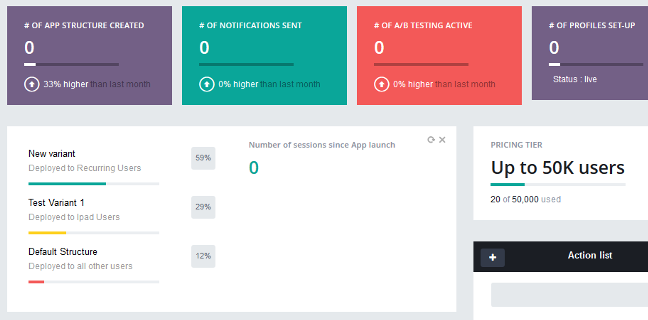
\includegraphics[width=12cm]{images/azetone/azetone_dashboard_flaws_for_kiwix_2015.png}
    \caption{Various flaws in Azetone's dashboard for a new project (2015)}
    \label{fig:azetone_dashboard_flaws_for_kiwix_2015}
\end{figure}

Comment from their CEO \emph{``FYI, by default our SDKs are reporting back to the servers with a delay which can be up to 15 hours (to minimize bandwidth and resource consumption)."}. However, during my limited evaluation no heatmaps appeared in their dashboard for our project.
